\documentclass[11pt]{article}
\usepackage[a4paper,margin=1in]{geometry}
\usepackage{amsmath,amssymb,amsthm}
\usepackage{tikz}
\usetikzlibrary{arrows.meta,positioning,shapes.misc}
\usepackage{xcolor}
\usepackage{booktabs}
\usepackage[hidelinks]{hyperref}
\hypersetup{pdftitle={A zero-sum selection game on matrices},pdfauthor={Vamshi Jandhyala}}

\newtheorem{theorem}{Theorem}
\newtheorem{lemma}[theorem]{Lemma}
\newtheorem{proposition}[theorem]{Proposition}
\newtheorem{corollary}[theorem]{Corollary}
\theoremstyle{definition}
\newtheorem{definition}[theorem]{Definition}
\theoremstyle{remark}
\newtheorem{remark}[theorem]{Remark}
\newtheorem*{question}{Question}

\newcommand{\R}{\mathbb{R}}
\newcommand{\Q}{\mathbb{Q}}
\definecolor{enemy}{RGB}{200,30,30}
\definecolor{you}{RGB}{0,90,200}

\title{A zero-sum selection game on matrices:\\ dimension, the order-three case, and complexity}
\author{Vamshi Jandhyala}
\date{}

\begin{document}
\maketitle

\begin{abstract}
Two players play on a real $n\times n$ matrix. The Enemy selects $i$ entries of row $i$ for each $i$; then You choose one selected entry in every row, and You win if the chosen entries sum to zero. V.~Lev asked on MathOverflow for a description of the matrices on which You win. We show that the winning matrices form a finite union of rational linear subspaces of dimension exactly $n(n+1)/2-1$, with the analogous statement for arbitrary row lengths and quotas; the proof is a short rank argument on zero-sum transversals. For $n=3$ we give a complete description, including five explicit families when every row has distinct entries. For general $n$, deciding whether a given integer matrix is winning is $\Pi_2^p$-complete, already when each row takes at most two values. So a description that can be checked in polynomial time does not exist unless the polynomial hierarchy collapses. The rank argument, the order-three classification and the two-valued normal form behind the hardness proof are formally verified in Lean.
\end{abstract}

\section{Introduction}

Here is the game, in the form Lev posed it~\cite{MO}. Two players, You and the Enemy, look at a real $n\times n$ matrix. First the Enemy selects one entry of the first row, two entries of the second row, and so on, down to all $n$ entries of the last row. Then You choose one selected entry in each row. You win if your $n$ entries sum to $0$. Which matrices are winning for You? Lev notes that the question arose in research, not as a puzzle; it is a question about which multisets of numbers force a zero sum against an adversary who removes options row by row.

For $n=2$ the answer is quick. The Enemy offers one entry $a$ of the first row and both entries $c,d$ of the second, so You need $-a\in\{c,d\}$ for each of the two possible $a$. Up to the order within rows the winning matrices are
\[
\begin{pmatrix} a & b\\ -a & -b\end{pmatrix},\qquad
\begin{pmatrix} a & a\\ -a & c\end{pmatrix}.
\]
For $n=3$ the first row is a single forced entry $a$, the third row is fully available, and all the play is in the middle row, where the Enemy hides one of three entries. Figure~\ref{fig:play} shows a winning matrix with distinct entries in every row:
\[
M=\begin{pmatrix}-1&-2&-3\\ 0&1&2\\ 0&1&3\end{pmatrix}.
\]
Whatever the Enemy does, You can reply: for $a=-1$ the second-row entries $0$ and $1$ both complete to zero ($-1+0+1=0$, $-1+1+0=0$), so hiding one of them does not help the Enemy, and similarly $a=-2$ is served by $1,2$ and $a=-3$ by $0,2$. The criterion is exactly this: every first-row entry must have two usable middle entries (Lemma~\ref{lem:crit}).

\begin{figure}[ht]
\centering
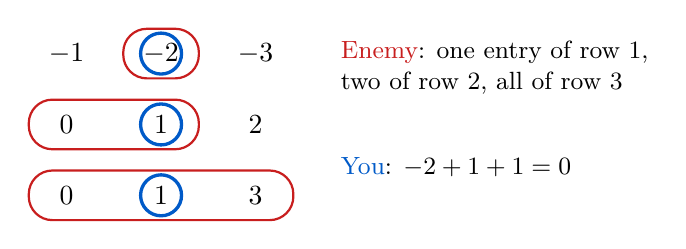
\begin{tikzpicture}[x=12mm,y=9mm]
\foreach \r/\a/\b/\c in {1/-1/-2/-3, 2/0/1/2, 3/0/1/3}{
  \node (m\r1) at (1,-\r) {$\a$}; \node (m\r2) at (2,-\r) {$\b$}; \node (m\r3) at (3,-\r) {$\c$};}
\draw[enemy,thick,rounded corners=3mm] (1.6,-0.65) rectangle (2.4,-1.35);
\draw[enemy,thick,rounded corners=3mm] (0.6,-1.65) rectangle (2.4,-2.35);
\draw[enemy,thick,rounded corners=3mm] (0.6,-2.65) rectangle (3.4,-3.35);
\foreach \n in {m12,m22,m32} \draw[you,very thick] (\n) circle (2.6mm);
\node[right,align=left,font=\small] at (3.8,-1.2) {\textcolor{enemy}{Enemy}: one entry of row 1,\\ two of row 2, all of row 3};
\node[right,align=left,font=\small] at (3.8,-2.6) {\textcolor{you}{You}: $-2+1+1=0$};
\end{tikzpicture}
\caption{One round on the matrix $M$. The Enemy's selection is boxed; Your zero-sum reply is circled.}
\label{fig:play}
\end{figure}

Lev asked for a description of all winning matrices. The question has been open on MathOverflow since 2023; the comments record the case $n=2$, examples for $n=3$ and $n=4$, and the observation that only the multiset of entries in each row matters~\cite{MO}. We prove three things.

\begin{theorem}\label{thm:dim}
The set of winning real $n\times n$ matrices is a finite union of linear subspaces of $\R^{n\times n}$ defined over $\Q$, and its dimension is exactly $\binom{n+1}2-1$. More generally, if row $i$ has $N_i$ entries and the Enemy selects $k_i$ of them ($1\le k_i\le N_i$), the winning set has dimension exactly $\sum_ik_i-1$.
\end{theorem}

\begin{theorem}\label{thm:three}
For $n=3$, a matrix is winning if and only if every first-row entry $a$ has at least two second-row positions $j$ with $-a-b_j$ in the third row. If every row has distinct entries, the winning matrices are, up to the order within rows and the translation $(A,B,C)\mapsto(A+u+v,\,B-u,\,C-v)$, exactly the five families of Table~\ref{tab:five}.
\end{theorem}

\begin{theorem}\label{thm:hard}
Deciding whether a given integer matrix is winning is $\Pi_2^p$-complete, even when every row has at most two distinct entries.
\end{theorem}

Theorem~\ref{thm:dim} says that winning has codimension exactly $\binom n2+1$, and Theorem~\ref{thm:hard} says that no simple test separates the pieces. The order-three answer, Theorem~\ref{thm:three}, shows what the pieces look like when they can be listed.

\section{Zero transversals}

A \emph{transversal} $t$ picks a position $t_i$ in each row; it is a \emph{zero transversal} of the matrix $a$ if $\sum_i a_{i,t_i}=0$. The Enemy's move is a product of position sets $S_1\times\dots\times S_n$ with $|S_i|=k_i$, a \emph{box}, and You win against it when some zero transversal lies in the box. So $a$ is winning exactly when its zero transversals meet every box.

It is convenient to turn the Enemy's selection around. Selecting $k_i$ of $N_i$ positions is the same as deleting the other $q_i=N_i-k_i$. So $a$ is winning if and only if every way of deleting at most $q_i$ positions from row $i$, for all $i$, leaves a zero transversal untouched.

For a transversal $t$ let $v_t\in\{0,1\}^{N}$, $N=\sum_iN_i$, be its incidence vector, with a $1$ in each chosen position. Then $t$ is a zero transversal of $a$ exactly when $v_t\cdot a=0$. Whether $a$ wins depends only on its set $H$ of zero transversals, and every $b$ with $v_t\cdot b=0$ for all $t\in H$ has at least those zero transversals. Hence the winning set is the union, over the finitely many sets $H$ of transversals that meet every box, of the subspaces $H^\perp=\{b: v_t\cdot b=0\ (t\in H)\}$. These are defined by equations with coefficients $0$ and $1$, so they are defined over $\Q$. This proves the first assertion of Theorem~\ref{thm:dim}; the content is the dimension.

\section{The dimension}

\begin{lemma}[rank lemma]\label{lem:rank}
If a set $H$ of transversals meets every box, then the vectors $v_t$, $t\in H$, span a space of dimension at least $1+\sum_i(N_i-k_i)$.
\end{lemma}

The idea is to delete positions one at a time, always a position used by a transversal that has survived so far, and to watch the span shrink (Figure~\ref{fig:delete}).

\begin{figure}[ht]
\centering
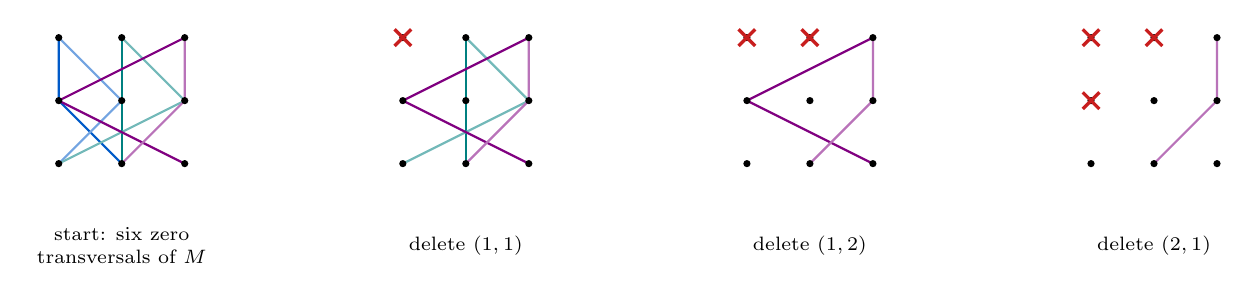
\begin{tikzpicture}[x=8mm,y=8mm]
\begin{scope}[xshift=0mm]
\draw[you,thick] (1,-1) -- (1,-2) -- (2,-3);
\draw[you!55,thick] (1,-1) -- (2,-2) -- (1,-3);
\draw[teal,thick] (2,-1) -- (2,-2) -- (2,-3);
\draw[teal!55,thick] (2,-1) -- (3,-2) -- (1,-3);
\draw[violet,thick] (3,-1) -- (1,-2) -- (3,-3);
\draw[violet!55,thick] (3,-1) -- (3,-2) -- (2,-3);
\fill[black] (1,-1) circle (1.3pt);
\fill[black] (2,-1) circle (1.3pt);
\fill[black] (3,-1) circle (1.3pt);
\fill[black] (1,-2) circle (1.3pt);
\fill[black] (2,-2) circle (1.3pt);
\fill[black] (3,-2) circle (1.3pt);
\fill[black] (1,-3) circle (1.3pt);
\fill[black] (2,-3) circle (1.3pt);
\fill[black] (3,-3) circle (1.3pt);
\node[font=\scriptsize,align=center] at (2,-4.3) {start: six zero\\transversals of $M$};
\end{scope}
\begin{scope}[xshift=1.15*38mm]
\draw[teal,thick] (2,-1) -- (2,-2) -- (2,-3);
\draw[teal!55,thick] (2,-1) -- (3,-2) -- (1,-3);
\draw[violet,thick] (3,-1) -- (1,-2) -- (3,-3);
\draw[violet!55,thick] (3,-1) -- (3,-2) -- (2,-3);
\fill[black] (1,-1) circle (1.3pt);
\fill[black] (2,-1) circle (1.3pt);
\fill[black] (3,-1) circle (1.3pt);
\fill[black] (1,-2) circle (1.3pt);
\fill[black] (2,-2) circle (1.3pt);
\fill[black] (3,-2) circle (1.3pt);
\fill[black] (1,-3) circle (1.3pt);
\fill[black] (2,-3) circle (1.3pt);
\fill[black] (3,-3) circle (1.3pt);
\node[cross out,draw=enemy,very thick,inner sep=2.4pt] at (1,-1) {};
\node[font=\scriptsize,align=center] at (2,-4.3) {delete $(1,1)$};
\end{scope}
\begin{scope}[xshift=1.15*76mm]
\draw[violet,thick] (3,-1) -- (1,-2) -- (3,-3);
\draw[violet!55,thick] (3,-1) -- (3,-2) -- (2,-3);
\fill[black] (1,-1) circle (1.3pt);
\fill[black] (2,-1) circle (1.3pt);
\fill[black] (3,-1) circle (1.3pt);
\fill[black] (1,-2) circle (1.3pt);
\fill[black] (2,-2) circle (1.3pt);
\fill[black] (3,-2) circle (1.3pt);
\fill[black] (1,-3) circle (1.3pt);
\fill[black] (2,-3) circle (1.3pt);
\fill[black] (3,-3) circle (1.3pt);
\node[cross out,draw=enemy,very thick,inner sep=2.4pt] at (1,-1) {};
\node[cross out,draw=enemy,very thick,inner sep=2.4pt] at (2,-1) {};
\node[font=\scriptsize,align=center] at (2,-4.3) {delete $(1,2)$};
\end{scope}
\begin{scope}[xshift=1.15*114mm]
\draw[violet!55,thick] (3,-1) -- (3,-2) -- (2,-3);
\fill[black] (1,-1) circle (1.3pt);
\fill[black] (2,-1) circle (1.3pt);
\fill[black] (3,-1) circle (1.3pt);
\fill[black] (1,-2) circle (1.3pt);
\fill[black] (2,-2) circle (1.3pt);
\fill[black] (3,-2) circle (1.3pt);
\fill[black] (1,-3) circle (1.3pt);
\fill[black] (2,-3) circle (1.3pt);
\fill[black] (3,-3) circle (1.3pt);
\node[cross out,draw=enemy,very thick,inner sep=2.4pt] at (1,-1) {};
\node[cross out,draw=enemy,very thick,inner sep=2.4pt] at (2,-1) {};
\node[cross out,draw=enemy,very thick,inner sep=2.4pt] at (1,-2) {};
\node[font=\scriptsize,align=center] at (2,-4.3) {delete $(2,1)$};
\end{scope}
\end{tikzpicture}
\caption{The deletion argument on the winning matrix $M$ of Figure~\ref{fig:play}. Rows are drawn horizontally; a line through one position per row is a zero transversal. The quotas $1,2,3$ allow two deletions in row~1 and one in row~2. Each deletion removes a position used by a surviving transversal, which removes that transversal's incidence vector from the span of the survivors, so the span drops in dimension. After all three deletions a transversal still survives, as it must, so the six vectors span at least $4$ dimensions.}
\label{fig:delete}
\end{figure}

\begin{proof}
Write $q_i=N_i-k_i$ and $q=\sum_iq_i$. By the reformulation above, whatever set of at most $q_i$ positions is deleted from each row, some transversal of $H$ avoids all deleted positions. Fix any order of $q$ deletions that deletes $q_i$ times from row $i$. Before each deletion, pick a surviving transversal $t$ and delete its position in the scheduled row. That position was not deleted before, since $t$ survived. The surviving transversals now all have a $0$ in that coordinate, while $v_t$ has a $1$ there, so the span of the surviving incidence vectors lies in a hyperplane that does not contain $v_t$, and its dimension drops by at least one. After $q$ deletions a transversal still survives, so the final span has dimension at least $1$. Hence the initial span has dimension at least $q+1$.
\end{proof}

\begin{proof}[Proof of Theorem~\ref{thm:dim}]
For each winning $a$ the subspace $H(a)^\perp$ through $a$ has dimension at most $N-(1+\sum_i(N_i-k_i))=\sum_ik_i-1$ by Lemma~\ref{lem:rank}. For the lower bound, put a value $b_i$ in $N_i-k_i+1$ positions of row $i$ and arbitrary values in the other $k_i-1$ positions, with $\sum_ib_i=0$. Any $k_i$ positions of row $i$ include one carrying $b_i$, so choosing those wins. The parameters are the $\sum_i(k_i-1)$ free entries and the $b_i$ subject to one equation, $\sum_ik_i-1$ in all, and they enter injectively. For the square game $\sum_ik_i=1+2+\dots+n$.
\end{proof}

The same argument bounds arithmetic rather than geometric freedom: for a winning matrix the entries span a $\Q$-vector space of dimension at most $\sum_ik_i-1$, because the $\Q$-linear map $c\mapsto c\cdot a$ on $\Q^N$ has at least $1+\sum_i(N_i-k_i)$ independent incidence vectors in its kernel. Also, any linear (or affine) family of winning matrices lies inside a single subspace $H^\perp$, because a real vector space is not a finite union of proper subspaces; so the bound applies to every such family.

\begin{remark}[distinct entries]\label{rem:paired}
The extremal family above repeats values. For even $n=2r$ the bound is also attained with distinct entries in every row. Take arbitrary rows $x_1,\dots,x_r$ and constants $c_1,\dots,c_r$ with $\sum c_i=0$, and let row $n+1-i$ be $c_i\mathbf 1-x_i$ (entries in any order). The Enemy selects $i$ positions of row $i$ and $n+1-i$ positions of row $n+1-i$; under the matching of positions these two sets meet, since $i+(n+1-i)>n$. Choosing a common position in each pair gives the sum $\sum_ic_i=0$. The family has $rn+r-1=\binom{n+1}2-1$ parameters, and generic choices give distinct entries. We do not know the answer for odd $n\ge3$ with distinct entries; for $n=3$ the maximum is $4$ (Section~\ref{sec:three}).
\end{remark}

\begin{remark}[a family from Hall's theorem]
Let row $i$ be $(r_i+c_1,\dots,r_i+c_n)$, in any order, with $\sum_ir_i+\sum_jc_j=0$. Label the positions of every row by $1,\dots,n$ through the $c_j$. The Enemy's selected label sets have sizes $1,2,\dots,n$, so any $m$ of them have a union of size at least $m$; by Hall's theorem they have a system of distinct representatives, which uses every label once and sums to $\sum_ir_i+\sum_jc_j=0$. This family has dimension $2n-2$ and, for $n=3$, is the generic member of the two-parameter family I below.
\end{remark}

\section{Order three}\label{sec:three}

\begin{lemma}\label{lem:crit}
A $3\times3$ matrix with rows $A,B,C$ is winning if and only if, for every entry $a$ of $A$, at least two positions $j$ of $B$ have $-a-b_j\in C$.
\end{lemma}

\begin{proof}
The Enemy offers one entry $a$ of $A$, two positions of $B$ and all of $C$. You can reply exactly when one of the two offered positions $j$ has $-a-b_j\in C$. Every pair of positions contains a usable one if and only if at most one position is unusable.
\end{proof}

When the second row has a repeated value $b$, the criterion reads $A\subseteq -b-C$, since the two copies of $b$ are usable together or not at all. The interesting case is three distinct second-row values, and Theorem~\ref{thm:three}'s five families come from it. Translating $B$ down by $u=\min B$, $C$ down by $v=\min C$ and $A$ up by $u+v$ preserves every sum $a+b+c$, so we may take
\[
B=(0,\,p,\,p+q),\qquad C=(0,\,r,\,r+s),\qquad p,q,r,s>0,
\]
when $B$ and $C$ have distinct entries. Then $a$ is usable at two positions exactly when $-a$ is a sum $x+y$ with $x\in B$, $y\in C$ in two different ways (two ways with the same $x$ would need the same $y$). Two such representations $x+y=x'+y'$ say that a difference of $B$ equals a difference of $C$.

\begin{lemma}[collisions]\label{lem:coll}
If $t$ has two representations $t=x+y$, then $t$ and the gaps satisfy one of the nine rows of Table~\ref{tab:coll}. Conversely each row gives two representations of its value.
\end{lemma}

\begin{table}[ht]
\centering
\begin{tabular}{lll}
\toprule
$B$-difference & $C$-difference & doubled value $t$\\
\midrule
$p$ & $r$ or $r+s$ & $p$\\
$p$ & $s$ & $p+r$\\
$q$ or $p+q$ & $r$ or $r+s$ & $p+q$\\
$q$ or $p+q$ & $s$ & $p+q+r$\\
\bottomrule
\end{tabular}
\caption{The nine coincidences of a difference of $B=(0,p,p+q)$ with a difference of $C=(0,r,r+s)$, and the value $t=x+y=x'+y'$ they double.}
\label{tab:coll}
\end{table}

\begin{proof}
Check the $3\times3$ choices of $(x,y)$ against $(x',y')$: a coincidence $x-x'=y'-y>0$ pairs one of the three positive differences $p,q,p+q$ of $B$ with one of $r,s,r+s$ of $C$, and in each case $t$ is read off as listed.
\end{proof}

\begin{table}[ht]
\centering
\begin{tabular}{cccc}
\toprule
Family & $A$ (up to order) & $B$ & $C$\\
\midrule
I & $(-p,\,-p-q,\,-2p-q)$ & $(0,p,p+q)$ & $(0,p,p+q)$\\
II & $(-h,-2h,-3h)$ & $(0,h,2h)$ & $(0,h,3h)$\\
III & $(-2h,-3h,-4h)$ & $(0,h,2h)$ & $(0,2h,3h)$\\
IV & $(-h,-2h,-3h)$ & $(0,h,3h)$ & $(0,h,2h)$\\
V & $(-2h,-3h,-4h)$ & $(0,2h,3h)$ & $(0,h,2h)$\\
\bottomrule
\end{tabular}
\caption{The winning $3\times3$ matrices with distinct entries in every row, normalised so that $\min B=\min C=0$; $p,q,h>0$. The matrix of Figure~\ref{fig:play} is family II with $h=1$.}
\label{tab:five}
\end{table}

\begin{proof}[Proof of Theorem~\ref{thm:three}, distinct entries]
The four possible doubled values are $p$, $p+r$, $p+q$, $p+q+r$, and a winning matrix with distinct first-row entries needs three distinct ones. Suppose, for instance, that $p$, $p+r$ and $p+q$ are all doubled. Then $p=s$ (the only way to double $p+r$), so $p=r+s$ is impossible and $p=r$; with $r=s=p$ the conditions for $p+q$ become $q=p$ or $q=2p$, which is family I with $q=p$ or family IV. The other three choices of three values are handled in the same way and give families I, II, III and V. Substituting each family's gaps into Table~\ref{tab:coll} shows that exactly three values are doubled, the negatives of the listed $A$, so the first row must be that triple. Conversely, Lemma~\ref{lem:coll} shows that each listed value is doubled, so each family wins.
\end{proof}

Without the distinctness assumption the same method gives a complete list. Up to the order within rows and the translation, every winning $3\times3$ matrix belongs to one of twelve linear families of dimensions $5,4,3$; as subspaces of $\R^9$ there are $1107$ maximal winning subspaces, $99$ of dimension $5$, $576$ of dimension $4$ and $432$ of dimension $3$. These numbers come from enumerating the minimal sets of zero transversals that meet every box, and two independent programs agree on them (Section~\ref{sec:verify}). The maximum $5=\binom42-1$ is Theorem~\ref{thm:dim}; with distinct entries in every row the maximum is $4$, attained by family I with the translation.

\section{Complexity}

For larger $n$ there is no comparably short list, and the reason is computational. The key case is a matrix whose rows take at most two values.

\begin{proposition}\label{prop:two}
Suppose every entry of row $i$ is $u_i$ or $w_i\ne u_i$, with $\alpha_i$ and $\beta_i$ copies. Call row $i$ \emph{universal} if $\alpha_i,\beta_i\ge k_i$, \emph{existential} if $\alpha_i,\beta_i<k_i$, and \emph{fixed} otherwise, with fixed value the one having at least $k_i$ copies. A constant row counts as fixed. Then the matrix is winning if and only if for every choice of $u_i$ or $w_i$ in the universal rows there is a choice in the existential rows such that these values and the fixed values sum to zero.
\end{proposition}

\begin{proof}
In a universal row the Enemy can select $k_i$ copies of either value, so he decides which value You get; in a fixed row he can always force the fixed value and can never exclude it; in an existential row any $k_i$ positions include both values. A selection of any other kind only offers You more, so the Enemy's best moves are exactly the choices of a value in each universal row, after which You choose freely in the existential rows.
\end{proof}

\begin{proof}[Proof of Theorem~\ref{thm:hard}]
Membership in $\Pi_2^p$ is the definition of the game: for all Enemy selections there exists a reply, and a reply is checked in polynomial time. For hardness we reduce from \textsc{Generalized Subset Sum}: given integers $u_1,\dots,u_p$, $w_1,\dots,w_q$ and $T$, decide whether for every $x\in\{0,1\}^p$ there is $y\in\{0,1\}^q$ with $\sum u_jx_j+\sum w_jy_j=T$. Its complement is $\Sigma_2^p$-complete~\cite{BKLPR,SU}, so it is $\Pi_2^p$-complete. We may drop indices with $u_j=0$ or $w_j=0$. Let $m=\max(p+1,q)$ and $n=2m$. Row $1$ is constant $-T$. Rows $2,\dots,p+1$ consist of $m$ zeros and $m$ copies of $u_{1},\dots,u_p$ respectively; since their quotas are at most $m$, they are universal. Rows $m+1,\dots,m+q$ consist of $m$ zeros and $m$ copies of $w_1,\dots,w_q$; their quotas exceed $m$, so they are existential. All other rows are zero, hence fixed. By Proposition~\ref{prop:two} the matrix is winning exactly when the subset-sum instance is true, and its size is polynomial in that of the instance.
\end{proof}

So recognising winning matrices is as hard as any problem at the second level of the polynomial hierarchy, and a polynomial-time recognisable description would give $\mathrm{P}=\Pi_2^p$. This does not exclude a structural description that is expensive to test, such as the finite union of Section~2, which can be generated from $n$ alone by exact linear algebra; it only rules out a cheap one.

\section{Questions}

\begin{question}
For odd $n\ge3$, what is the largest dimension of a family of winning matrices with distinct entries in every row? For $n=3$ it is $4$, one less than the unrestricted maximum.
\end{question}

\begin{question}
How many maximal winning subspaces are there for $n=4$? For $n=3$ there are $1107$, in twelve orbits under permutations within rows.
\end{question}

\section{Verification}\label{sec:verify}

Lemma~\ref{lem:rank} and Theorem~\ref{thm:dim} (both bounds, for arbitrary row lengths and quotas, and the finite-union statement), Lemma~\ref{lem:crit}, Lemma~\ref{lem:coll} and its converse, the distinct-entry classification in normalised form, and Proposition~\ref{prop:two} are formally verified in Lean~4 with Mathlib~\cite{mathlib}, using only the standard axioms. Not formalised are the bookkeeping of the hardness reduction (which rows are universal), the twelve families and the count $1107$, and the two remarks of Section~3. A program sharing no code with the formal proofs or with the programs that found these results checks, by playing the game literally: the criterion on all $592{,}704$ matrices with sorted rows from $\{-3,\dots,3\}$; the five families against all matrices with distinct rows from $\{-4,\dots,4\}$; the count $1107$ by its own enumeration; Proposition~\ref{prop:two} on random two-valued matrices; the reduction on random subset-sum instances, true and false; and the families of the remarks. The code is at \url{https://github.com/jvvk/mathematics}.

\section*{Acknowledgement}

The author used two AI assistants, Codex (OpenAI) and Claude Opus~5.5 (Anthropic). Codex found the results of this paper, wrote the programs that found the order-three components and the first formal proof of the rank lemma. Claude formalised the order-three classification and the two-valued normal form, wrote the independent checking program and drafted the text. The author directed the work, checked the results and is responsible for the contents.

\begin{thebibliography}{9}
\bibitem{BKLPR} P. Berman, M. Karpinski, L. L. Larmore, W. Plandowski and W. Rytter, On the complexity of pattern matching for highly compressed two-dimensional texts, in \emph{Combinatorial Pattern Matching (CPM 1997)}, Lecture Notes in Comput. Sci. \textbf{1264}, Springer, 1997, 40--51.
\bibitem{MO} V. Lev, A matrix / zero forcing game, MathOverflow question 453809 (2023), \url{https://mathoverflow.net/q/453809}.
\bibitem{mathlib} The mathlib Community, The Lean mathematical library, in \emph{Proceedings of the 9th ACM SIGPLAN International Conference on Certified Programs and Proofs} (2020), 367--381.
\bibitem{SU} M. Schaefer and C. Umans, Completeness in the polynomial-time hierarchy: a compendium, version of 5 October 2008, problem SP2, \url{https://ovid.cs.depaul.edu/documents/phcom.pdf}.
\end{thebibliography}

\end{document}
